% Gerado por ais.cli.build_trip_gallery_pdf a partir de viagens/README.md. NÃO EDITAR À MÃO.
% Compilar a partir de viagens/.
\documentclass[a4paper,11pt]{article}
\usepackage[utf8]{inputenc}
\usepackage[T1]{fontenc}
\usepackage{times}
\usepackage[hmargin=2cm,vmargin=1.5cm]{geometry}
\usepackage{graphicx}
\usepackage{booktabs}
\usepackage[hidelinks]{hyperref}
% Sem padrões de hifenização portugueses: não partir palavras.
\hyphenpenalty=10000
\exhyphenpenalty=10000
\emergencystretch=3em
\setlength{\parindent}{0pt}
\setlength{\parskip}{6pt}

\title{Viagens: o que cada modelo previu}
\author{Dinis Soveral Botelho Rosa\\University of Coimbra / Department of Informatics Engineering}
\date{}
\begin{document}
\maketitle

Uma imagem por viagem dos conjuntos de teste e de validação, com a classe de cada ponto: \textbf{azul} é navegação e \textbf{laranja} é pesca. O método e a discussão estão no relatório (\texttt{latex/relatorio\_pt.tex}).

{\centering\small
\begin{tabular}{lp{0.62\linewidth}}
\toprule
Linha & O que é \\
\midrule
real & classe anotada no conjunto de dados \\
baseline & CNN 1D sobre a viagem completa \\
J0 & a mesma CNN em janelas de 64 pontos, sem sobreposição \\
J50 & a mesma CNN em janelas de 64 pontos, com 50\,\% de sobreposição \\
baseline + pós-processamento & a baseline depois de um filtro gaussiano de 301 pontos sobre as probabilidades \\
\bottomrule
\end{tabular}\par}

\section*{Como ler estes resultados}

\begin{itemize}
\item O conjunto de \textbf{teste} serviu para escolher épocas, limiares e a janela do filtro: os seus resultados são \textbf{otimistas}.
\item Na \textbf{validação}, só a baseline é a medição final. O filtro \textbf{não é uma medição independente}: antes dele aplicou-se à validação uma versão de 13 pontos. J0 e J50 não foram medidos neste conjunto.
\item O filtro aplica-se só à baseline. Estas imagens servem para ver, não para escolher valores.
\item O eixo horizontal conta pontos e não tempo. Nas viagens longas há vários pontos por píxel, e um bloco muito curto aparece esbatido ou quase não se vê: a tabela conta todos os segmentos.
\item Em cada conjunto, as viagens estão por ordem crescente de exatidão da baseline.
\end{itemize}

Dados: Song Wu, \emph{Detailed Labelled Fishing Trajectories from AIS}, Zenodo, \href{https://doi.org/10.5281/zenodo.7283281}{10.5281/zenodo.7283281}, \href{https://creativecommons.org/licenses/by/4.0/}{CC BY 4.0}. As imagens são derivadas desses dados e das previsões deste projeto.

\textbf{Conjuntos:} \hyperlink{teste}{Teste (18 viagens)} \textperiodcentered{} \hyperlink{validacao}{Validação (18 viagens)}

\clearpage
\hypertarget{teste}{}
\section*{Teste}

{\raggedright Viagens: \hyperlink{220006000-2}{220006000-2} \textperiodcentered{} \hyperlink{219001624-2}{219001624-2} \textperiodcentered{} \hyperlink{219028381-4}{219028381-4} \textperiodcentered{} \hyperlink{232020276-3}{232020276-3} \textperiodcentered{} \hyperlink{219004596-2}{219004596-2} \textperiodcentered{} \hyperlink{232020276-2}{232020276-2} \textperiodcentered{} \hyperlink{219002409-2}{219002409-2} \textperiodcentered{} \hyperlink{219001682-2}{219001682-2} \textperiodcentered{} \hyperlink{219000855-4}{219000855-4} \textperiodcentered{} \hyperlink{219025739-4}{219025739-4} \textperiodcentered{} \hyperlink{219025740-6}{219025740-6} \textperiodcentered{} \hyperlink{219000855-3}{219000855-3} \textperiodcentered{} \hyperlink{220349000-3}{220349000-3} \textperiodcentered{} \hyperlink{219007027-3}{219007027-3} \textperiodcentered{} \hyperlink{219005671-2}{219005671-2} \textperiodcentered{} \hyperlink{219004203-3}{219004203-3} \textperiodcentered{} \hyperlink{219015617-2}{219015617-2} \textperiodcentered{} \hyperlink{219001604-2}{219001604-2}\par}\medskip

\par\smallskip\noindent\begin{minipage}{\linewidth}\setlength{\parskip}{3pt}
\hypertarget{220006000-2}{}\textbf{\large 220006000-2}\par

{\centering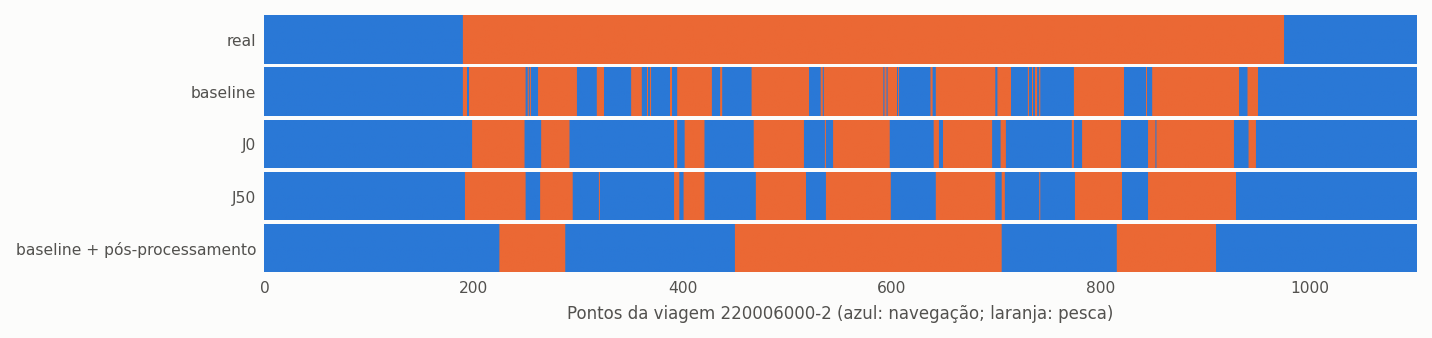
\includegraphics[width=0.9\linewidth]{teste/220006000-2.png}\par}

1 102 pontos; segmentos de pesca reais: 1.

{\centering\small
\begin{tabular}{lrr}
\toprule
Linha & Exatidão & Segmentos de pesca previstos \\
\midrule
baseline & 74,0\,\% & 29 \\
J0 & 63,8\,\% & 15 \\
J50 & 66,4\,\% & 12 \\
baseline + pós-processamento & 66,2\,\% & 3 \\
\bottomrule
\end{tabular}\par}

\end{minipage}
\par

\par\smallskip\noindent\begin{minipage}{\linewidth}\setlength{\parskip}{3pt}
\hypertarget{219001624-2}{}\textbf{\large 219001624-2}\par

{\centering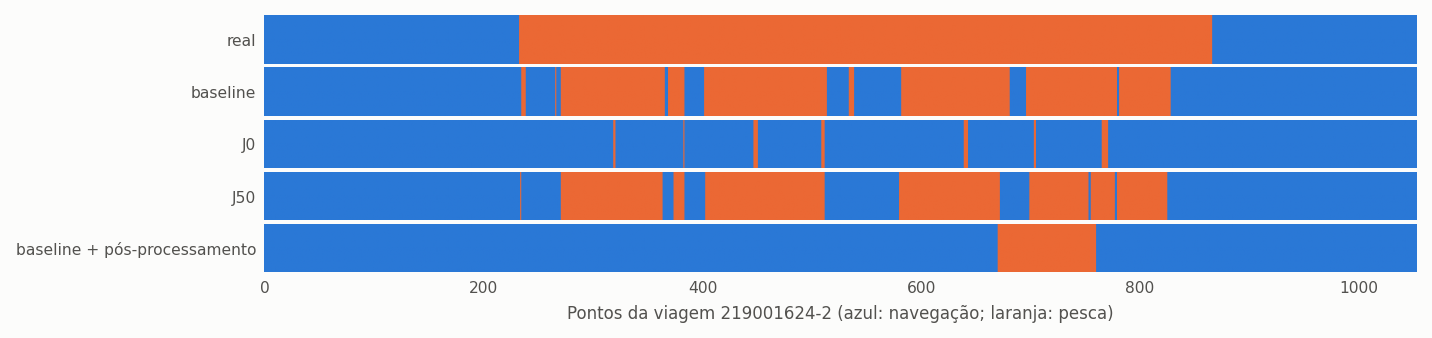
\includegraphics[width=0.9\linewidth]{teste/219001624-2.png}\par}

1 053 pontos; segmentos de pesca reais: 1.

{\centering\small
\begin{tabular}{lrr}
\toprule
Linha & Exatidão & Segmentos de pesca previstos \\
\midrule
baseline & 83,7\,\% & 9 \\
J0 & 42,0\,\% & 7 \\
J50 & 80,4\,\% & 8 \\
baseline + pós-processamento & 48,4\,\% & 1 \\
\bottomrule
\end{tabular}\par}

\end{minipage}
\par

\par\smallskip\noindent\begin{minipage}{\linewidth}\setlength{\parskip}{3pt}
\hypertarget{219028381-4}{}\textbf{\large 219028381-4}\par

{\centering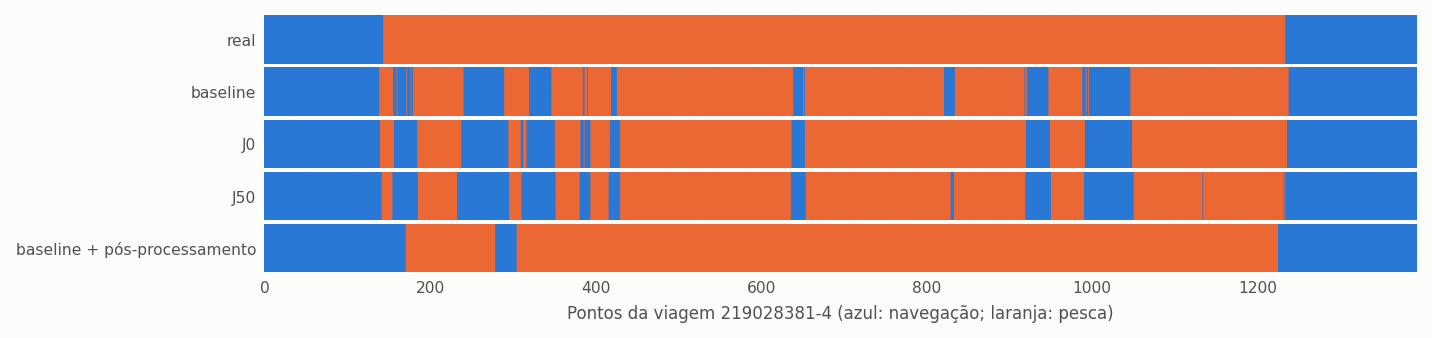
\includegraphics[width=0.9\linewidth]{teste/219028381-4.png}\par}

1 392 pontos; segmentos de pesca reais: 1.

{\centering\small
\begin{tabular}{lrr}
\toprule
Linha & Exatidão & Segmentos de pesca previstos \\
\midrule
baseline & 83,8\,\% & 18 \\
J0 & 81,8\,\% & 11 \\
J50 & 80,0\,\% & 12 \\
baseline + pós-processamento & 95,5\,\% & 2 \\
\bottomrule
\end{tabular}\par}

\end{minipage}
\par

\par\smallskip\noindent\begin{minipage}{\linewidth}\setlength{\parskip}{3pt}
\hypertarget{232020276-3}{}\textbf{\large 232020276-3}\par

{\centering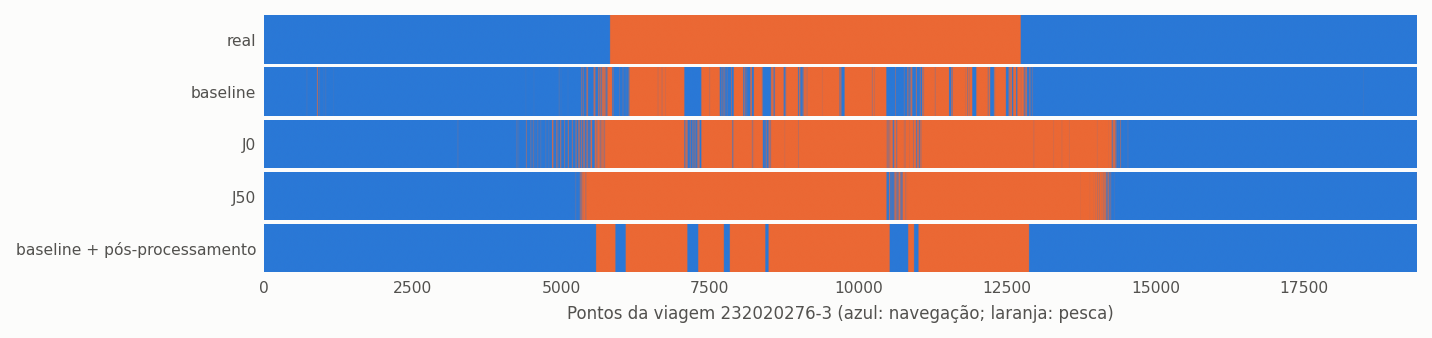
\includegraphics[width=0.9\linewidth]{teste/232020276-3.png}\par}

19 390 pontos; segmentos de pesca reais: 1.

{\centering\small
\begin{tabular}{lrr}
\toprule
Linha & Exatidão & Segmentos de pesca previstos \\
\midrule
baseline & 87,5\,\% & 121 \\
J0 & 87,3\,\% & 123 \\
J50 & 89,2\,\% & 52 \\
baseline + pós-processamento & 93,4\,\% & 7 \\
\bottomrule
\end{tabular}\par}

\end{minipage}
\par

\par\smallskip\noindent\begin{minipage}{\linewidth}\setlength{\parskip}{3pt}
\hypertarget{219004596-2}{}\textbf{\large 219004596-2}\par

{\centering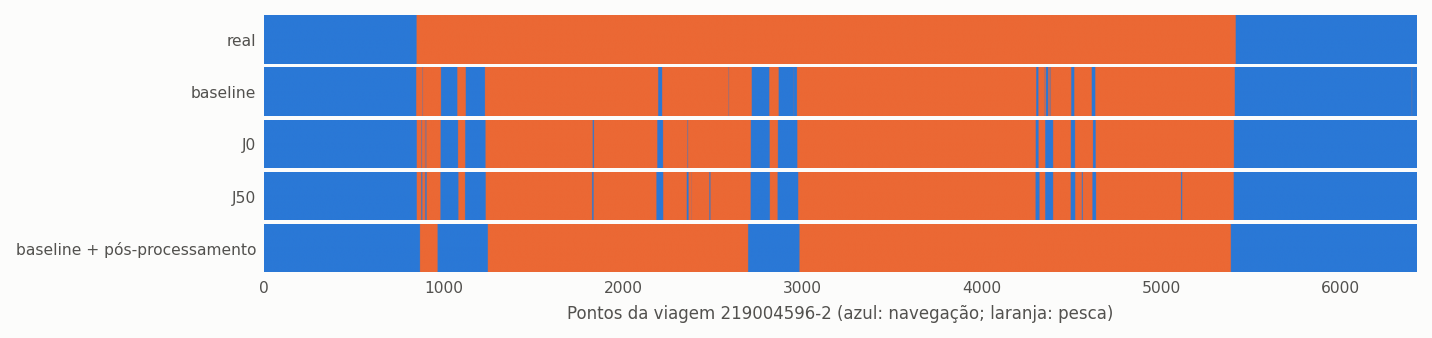
\includegraphics[width=0.9\linewidth]{teste/219004596-2.png}\par}

6 423 pontos; segmentos de pesca reais: 1.

{\centering\small
\begin{tabular}{lrr}
\toprule
Linha & Exatidão & Segmentos de pesca previstos \\
\midrule
baseline & 92,2\,\% & 17 \\
J0 & 91,0\,\% & 15 \\
J50 & 89,9\,\% & 19 \\
baseline + pós-processamento & 90,5\,\% & 3 \\
\bottomrule
\end{tabular}\par}

\end{minipage}
\par

\par\smallskip\noindent\begin{minipage}{\linewidth}\setlength{\parskip}{3pt}
\hypertarget{232020276-2}{}\textbf{\large 232020276-2}\par

{\centering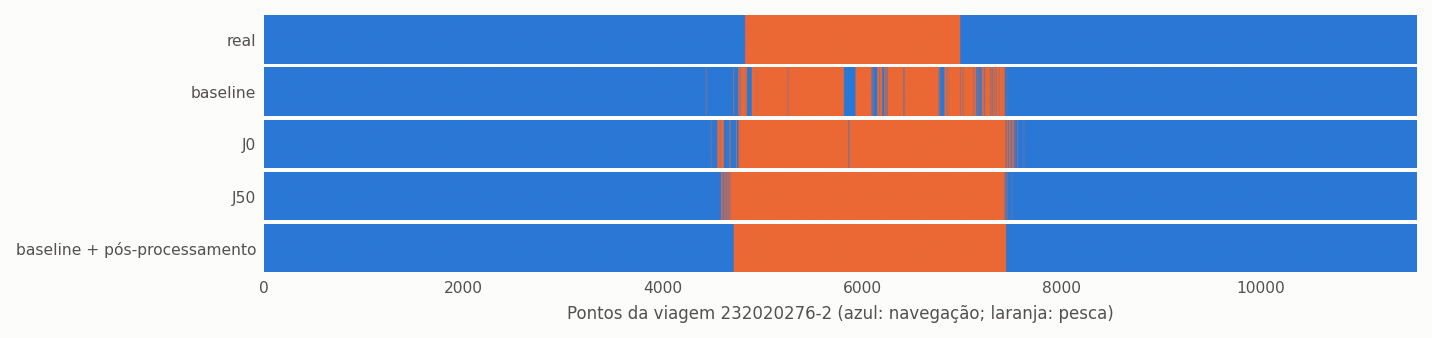
\includegraphics[width=0.9\linewidth]{teste/232020276-2.png}\par}

11 558 pontos; segmentos de pesca reais: 1.

{\centering\small
\begin{tabular}{lrr}
\toprule
Linha & Exatidão & Segmentos de pesca previstos \\
\midrule
baseline & 93,4\,\% & 48 \\
J0 & 94,1\,\% & 20 \\
J50 & 94,3\,\% & 18 \\
baseline + pós-processamento & 95,0\,\% & 1 \\
\bottomrule
\end{tabular}\par}

\end{minipage}
\par

\par\smallskip\noindent\begin{minipage}{\linewidth}\setlength{\parskip}{3pt}
\hypertarget{219002409-2}{}\textbf{\large 219002409-2}\par

{\centering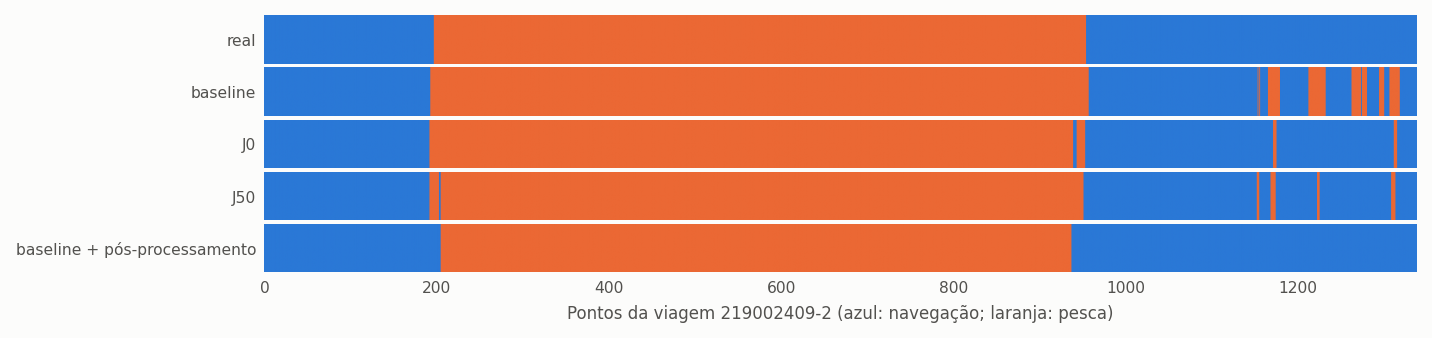
\includegraphics[width=0.9\linewidth]{teste/219002409-2.png}\par}

1 338 pontos; segmentos de pesca reais: 1.

{\centering\small
\begin{tabular}{lrr}
\toprule
Linha & Exatidão & Segmentos de pesca previstos \\
\midrule
baseline & 94,2\,\% & 9 \\
J0 & 98,7\,\% & 4 \\
J50 & 98,0\,\% & 6 \\
baseline + pós-processamento & 98,1\,\% & 1 \\
\bottomrule
\end{tabular}\par}

\end{minipage}
\par

\par\smallskip\noindent\begin{minipage}{\linewidth}\setlength{\parskip}{3pt}
\hypertarget{219001682-2}{}\textbf{\large 219001682-2}\par

{\centering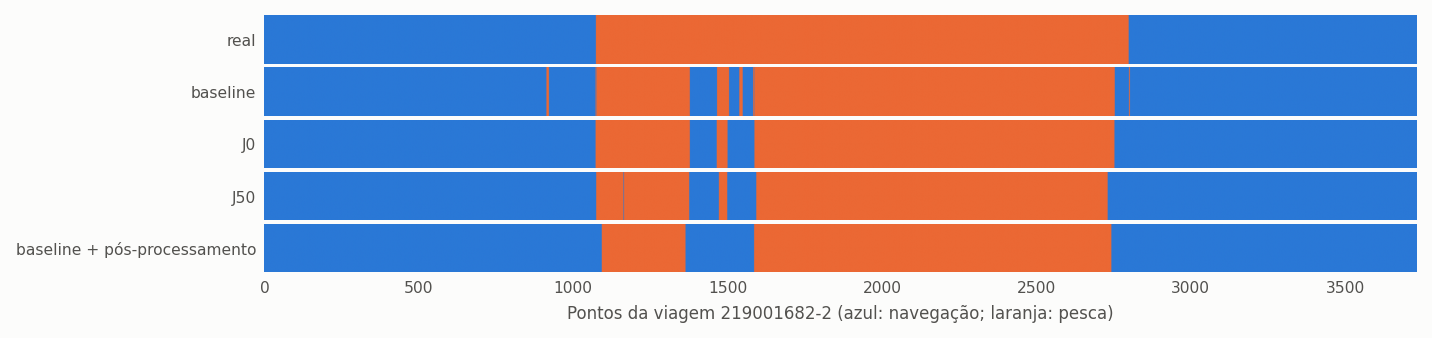
\includegraphics[width=0.9\linewidth]{teste/219001682-2.png}\par}

3 731 pontos; segmentos de pesca reais: 1.

{\centering\small
\begin{tabular}{lrr}
\toprule
Linha & Exatidão & Segmentos de pesca previstos \\
\midrule
baseline & 94,3\,\% & 8 \\
J0 & 94,1\,\% & 3 \\
J50 & 93,0\,\% & 4 \\
baseline + pós-processamento & 92,0\,\% & 2 \\
\bottomrule
\end{tabular}\par}

\end{minipage}
\par

\par\smallskip\noindent\begin{minipage}{\linewidth}\setlength{\parskip}{3pt}
\hypertarget{219000855-4}{}\textbf{\large 219000855-4}\par

{\centering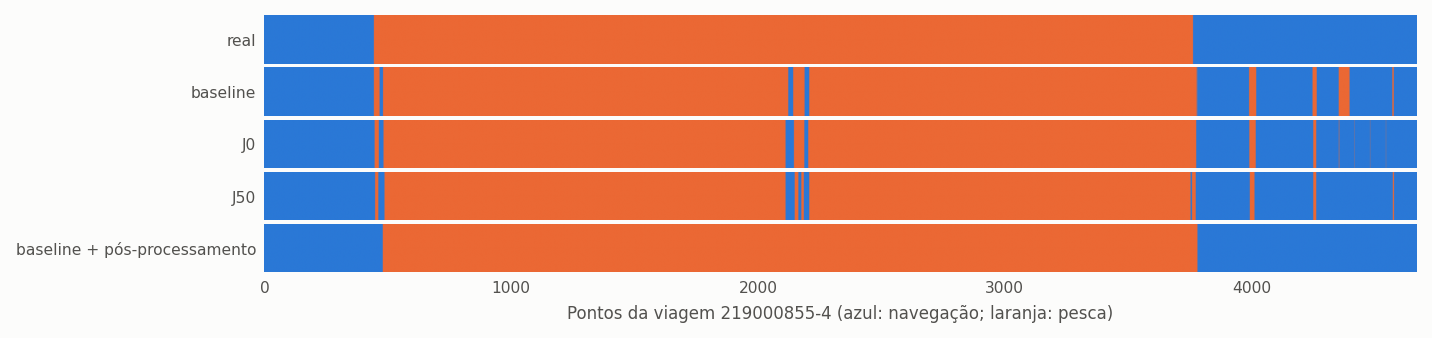
\includegraphics[width=0.9\linewidth]{teste/219000855-4.png}\par}

4 669 pontos; segmentos de pesca reais: 1.

{\centering\small
\begin{tabular}{lrr}
\toprule
Linha & Exatidão & Segmentos de pesca previstos \\
\midrule
baseline & 96,5\,\% & 9 \\
J0 & 97,3\,\% & 11 \\
J50 & 96,7\,\% & 9 \\
baseline + pós-processamento & 98,8\,\% & 1 \\
\bottomrule
\end{tabular}\par}

\end{minipage}
\par

\par\smallskip\noindent\begin{minipage}{\linewidth}\setlength{\parskip}{3pt}
\hypertarget{219025739-4}{}\textbf{\large 219025739-4}\par

{\centering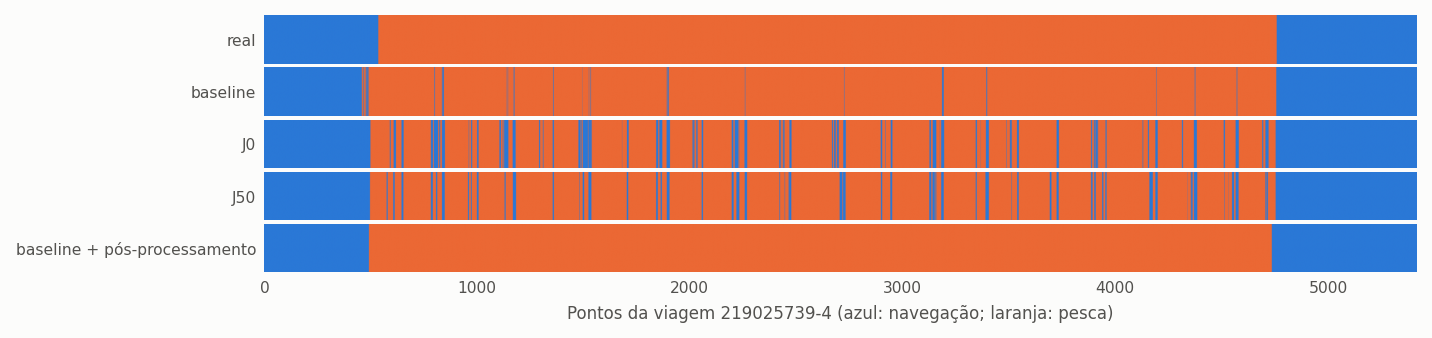
\includegraphics[width=0.9\linewidth]{teste/219025739-4.png}\par}

5 416 pontos; segmentos de pesca reais: 1.

{\centering\small
\begin{tabular}{lrr}
\toprule
Linha & Exatidão & Segmentos de pesca previstos \\
\midrule
baseline & 97,7\,\% & 28 \\
J0 & 88,6\,\% & 78 \\
J50 & 91,0\,\% & 59 \\
baseline + pós-processamento & 98,8\,\% & 1 \\
\bottomrule
\end{tabular}\par}

\end{minipage}
\par

\par\smallskip\noindent\begin{minipage}{\linewidth}\setlength{\parskip}{3pt}
\hypertarget{219025740-6}{}\textbf{\large 219025740-6}\par

{\centering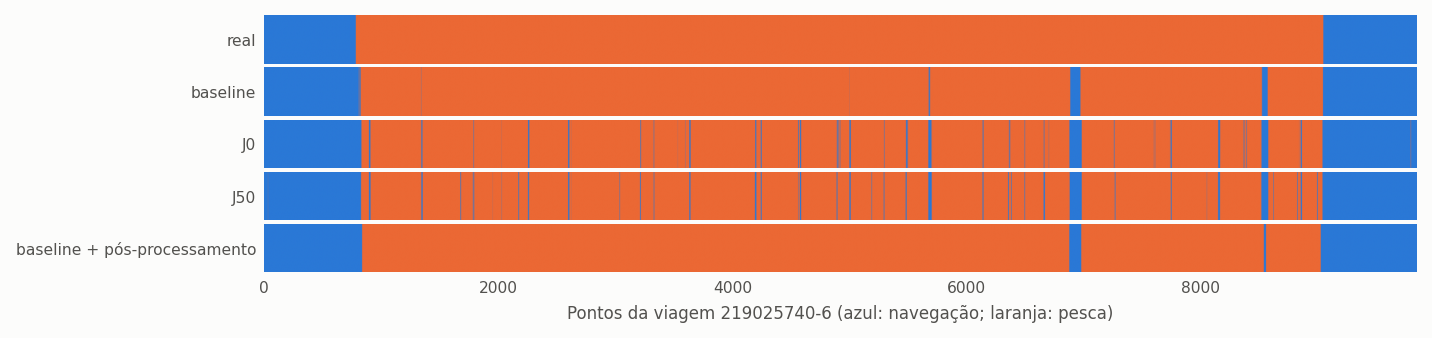
\includegraphics[width=0.9\linewidth]{teste/219025740-6.png}\par}

9 846 pontos; segmentos de pesca reais: 1.

{\centering\small
\begin{tabular}{lrr}
\toprule
Linha & Exatidão & Segmentos de pesca previstos \\
\midrule
baseline & 98,1\,\% & 9 \\
J0 & 95,1\,\% & 49 \\
J50 & 94,9\,\% & 44 \\
baseline + pós-processamento & 98,0\,\% & 3 \\
\bottomrule
\end{tabular}\par}

\end{minipage}
\par

\par\smallskip\noindent\begin{minipage}{\linewidth}\setlength{\parskip}{3pt}
\hypertarget{219000855-3}{}\textbf{\large 219000855-3}\par

{\centering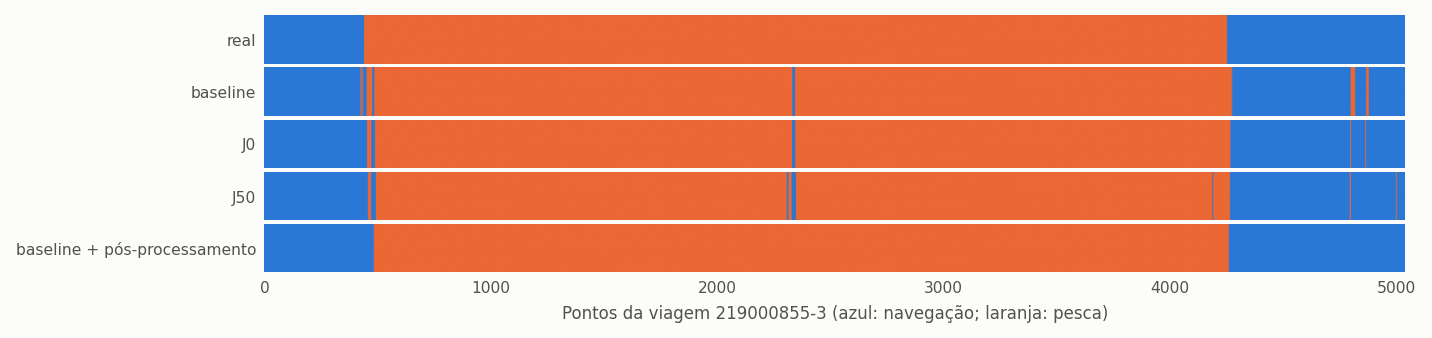
\includegraphics[width=0.9\linewidth]{teste/219000855-3.png}\par}

5 039 pontos; segmentos de pesca reais: 1.

{\centering\small
\begin{tabular}{lrr}
\toprule
Linha & Exatidão & Segmentos de pesca previstos \\
\midrule
baseline & 98,1\,\% & 9 \\
J0 & 98,7\,\% & 5 \\
J50 & 98,2\,\% & 7 \\
baseline + pós-processamento & 99,0\,\% & 1 \\
\bottomrule
\end{tabular}\par}

\end{minipage}
\par

\par\smallskip\noindent\begin{minipage}{\linewidth}\setlength{\parskip}{3pt}
\hypertarget{220349000-3}{}\textbf{\large 220349000-3}\par

{\centering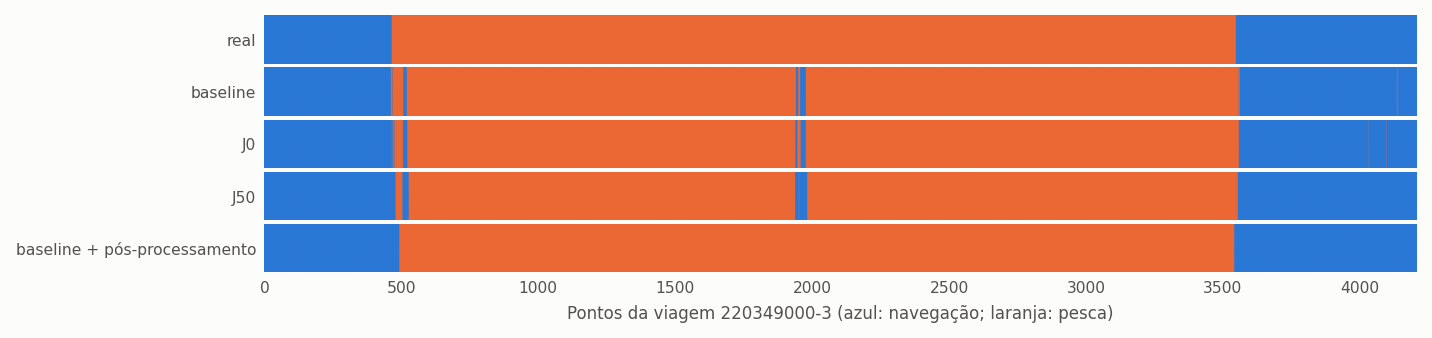
\includegraphics[width=0.9\linewidth]{teste/220349000-3.png}\par}

4 207 pontos; segmentos de pesca reais: 1.

{\centering\small
\begin{tabular}{lrr}
\toprule
Linha & Exatidão & Segmentos de pesca previstos \\
\midrule
baseline & 98,5\,\% & 7 \\
J0 & 98,6\,\% & 8 \\
J50 & 97,9\,\% & 4 \\
baseline + pós-processamento & 99,2\,\% & 1 \\
\bottomrule
\end{tabular}\par}

\end{minipage}
\par

\par\smallskip\noindent\begin{minipage}{\linewidth}\setlength{\parskip}{3pt}
\hypertarget{219007027-3}{}\textbf{\large 219007027-3}\par

{\centering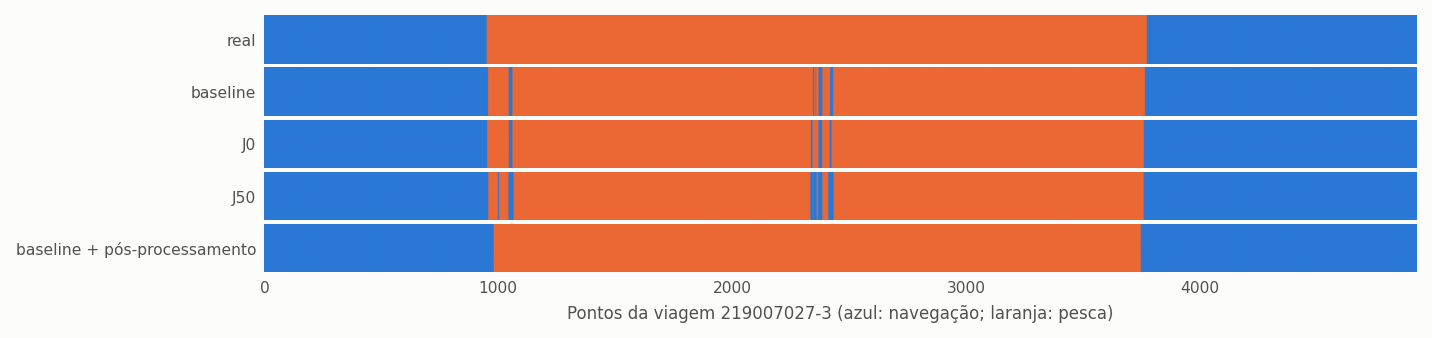
\includegraphics[width=0.9\linewidth]{teste/219007027-3.png}\par}

4 925 pontos; segmentos de pesca reais: 1.

{\centering\small
\begin{tabular}{lrr}
\toprule
Linha & Exatidão & Segmentos de pesca previstos \\
\midrule
baseline & 98,7\,\% & 6 \\
J0 & 98,8\,\% & 5 \\
J50 & 97,6\,\% & 7 \\
baseline + pós-processamento & 98,9\,\% & 1 \\
\bottomrule
\end{tabular}\par}

\end{minipage}
\par

\par\smallskip\noindent\begin{minipage}{\linewidth}\setlength{\parskip}{3pt}
\hypertarget{219005671-2}{}\textbf{\large 219005671-2}\par

{\centering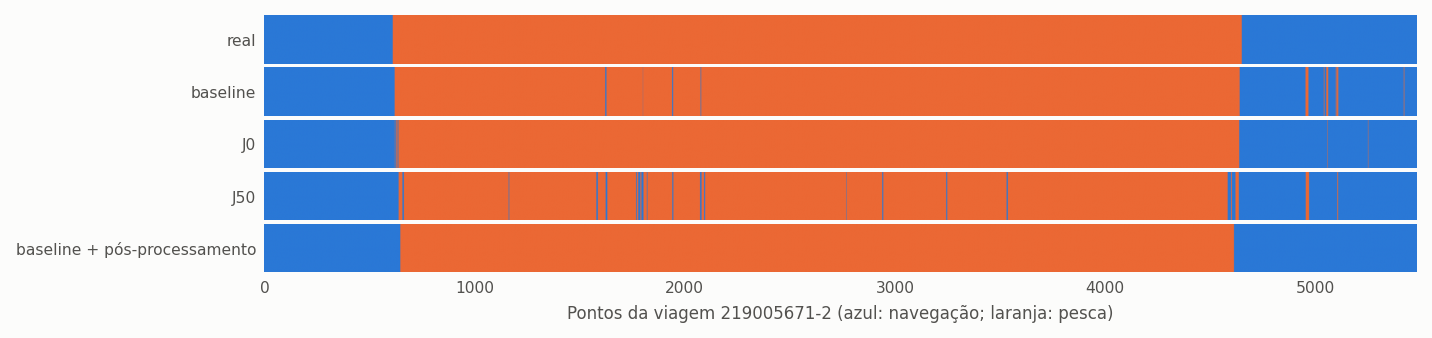
\includegraphics[width=0.9\linewidth]{teste/219005671-2.png}\par}

5 481 pontos; segmentos de pesca reais: 1.

{\centering\small
\begin{tabular}{lrr}
\toprule
Linha & Exatidão & Segmentos de pesca previstos \\
\midrule
baseline & 98,7\,\% & 14 \\
J0 & 99,4\,\% & 6 \\
J50 & 96,7\,\% & 21 \\
baseline + pós-processamento & 98,7\,\% & 1 \\
\bottomrule
\end{tabular}\par}

\end{minipage}
\par

\par\smallskip\noindent\begin{minipage}{\linewidth}\setlength{\parskip}{3pt}
\hypertarget{219004203-3}{}\textbf{\large 219004203-3}\par

{\centering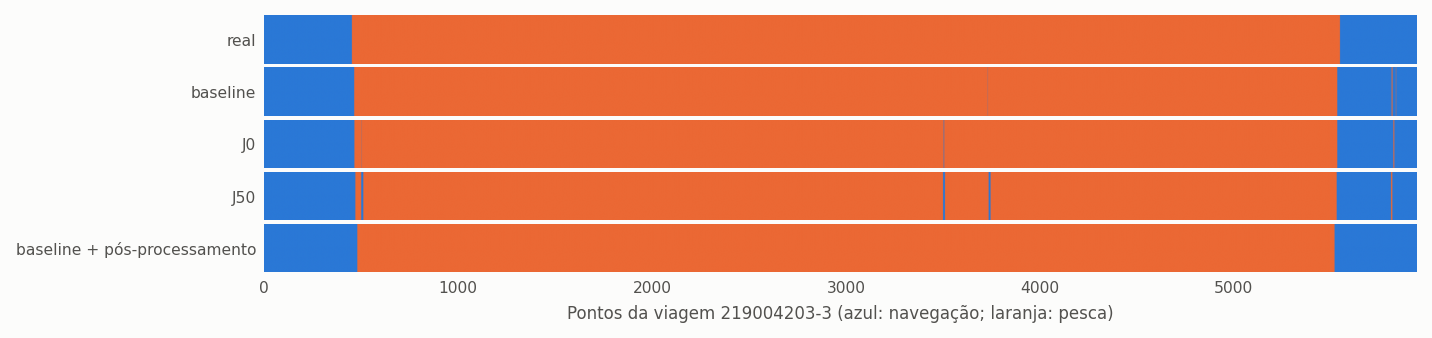
\includegraphics[width=0.9\linewidth]{teste/219004203-3.png}\par}

5 943 pontos; segmentos de pesca reais: 1.

{\centering\small
\begin{tabular}{lrr}
\toprule
Linha & Exatidão & Segmentos de pesca previstos \\
\midrule
baseline & 99,4\,\% & 4 \\
J0 & 99,4\,\% & 5 \\
J50 & 98,8\,\% & 5 \\
baseline + pós-processamento & 99,1\,\% & 1 \\
\bottomrule
\end{tabular}\par}

\end{minipage}
\par

\par\smallskip\noindent\begin{minipage}{\linewidth}\setlength{\parskip}{3pt}
\hypertarget{219015617-2}{}\textbf{\large 219015617-2}\par

{\centering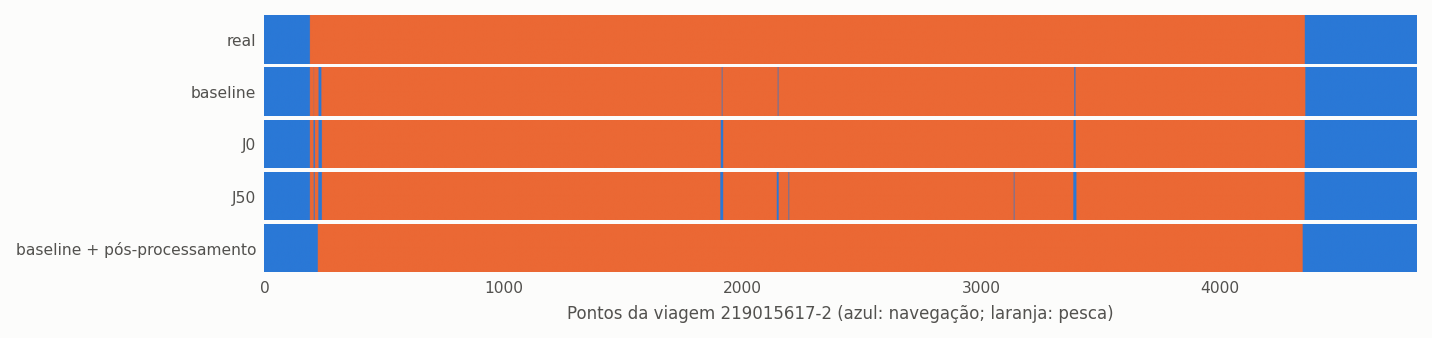
\includegraphics[width=0.9\linewidth]{teste/219015617-2.png}\par}

4 821 pontos; segmentos de pesca reais: 1.

{\centering\small
\begin{tabular}{lrr}
\toprule
Linha & Exatidão & Segmentos de pesca previstos \\
\midrule
baseline & 99,5\,\% & 6 \\
J0 & 99,2\,\% & 5 \\
J50 & 98,8\,\% & 8 \\
baseline + pós-processamento & 99,1\,\% & 1 \\
\bottomrule
\end{tabular}\par}

\end{minipage}
\par

\par\smallskip\noindent\begin{minipage}{\linewidth}\setlength{\parskip}{3pt}
\hypertarget{219001604-2}{}\textbf{\large 219001604-2}\par

{\centering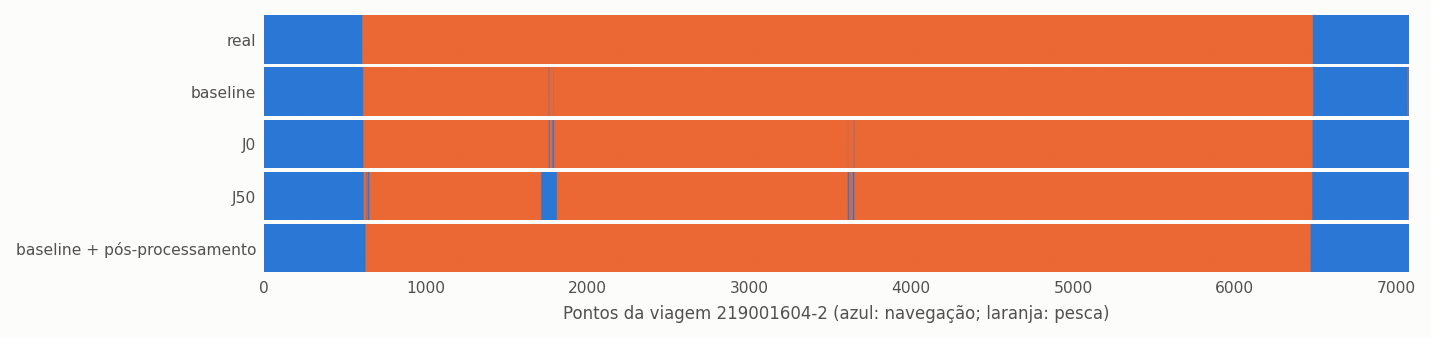
\includegraphics[width=0.9\linewidth]{teste/219001604-2.png}\par}

7 075 pontos; segmentos de pesca reais: 1.

{\centering\small
\begin{tabular}{lrr}
\toprule
Linha & Exatidão & Segmentos de pesca previstos \\
\midrule
baseline & 99,8\,\% & 7 \\
J0 & 99,6\,\% & 7 \\
J50 & 97,9\,\% & 8 \\
baseline + pós-processamento & 99,5\,\% & 1 \\
\bottomrule
\end{tabular}\par}

\end{minipage}
\par

\clearpage
\hypertarget{validacao}{}
\section*{Validação}

{\raggedright Viagens: \hyperlink{219020187-4}{219020187-4} \textperiodcentered{} \hyperlink{220204000-3}{220204000-3} \textperiodcentered{} \hyperlink{219012671-2}{219012671-2} \textperiodcentered{} \hyperlink{220335000-2}{220335000-2} \textperiodcentered{} \hyperlink{219004343-1}{219004343-1} \textperiodcentered{} \hyperlink{219796000-2}{219796000-2} \textperiodcentered{} \hyperlink{219007027-2}{219007027-2} \textperiodcentered{} \hyperlink{219004128-2}{219004128-2} \textperiodcentered{} \hyperlink{220307000-3}{220307000-3} \textperiodcentered{} \hyperlink{219027026-2}{219027026-2} \textperiodcentered{} \hyperlink{211477000-2}{211477000-2} \textperiodcentered{} \hyperlink{219009738-2}{219009738-2} \textperiodcentered{} \hyperlink{219709000-2}{219709000-2} \textperiodcentered{} \hyperlink{220307000-4}{220307000-4} \textperiodcentered{} \hyperlink{219025740-2}{219025740-2} \textperiodcentered{} \hyperlink{220356000-3}{220356000-3} \textperiodcentered{} \hyperlink{219004128-4}{219004128-4} \textperiodcentered{} \hyperlink{220351000-2}{220351000-2}\par}\medskip

\par\smallskip\noindent\begin{minipage}{\linewidth}\setlength{\parskip}{3pt}
\hypertarget{219020187-4}{}\textbf{\large 219020187-4}\par

{\centering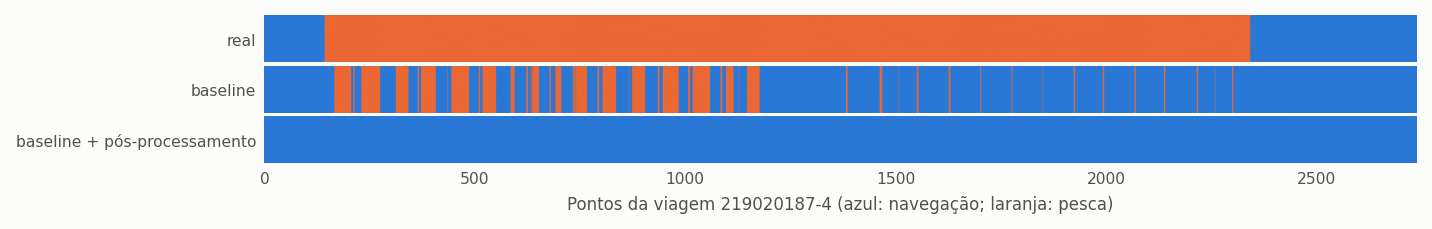
\includegraphics[width=0.9\linewidth]{validacao/219020187-4.png}\par}

2 738 pontos; segmentos de pesca reais: 1.

{\centering\small
\begin{tabular}{lrr}
\toprule
Linha & Exatidão & Segmentos de pesca previstos \\
\midrule
baseline & 40,4\,\% & 49 \\
baseline + pós-processamento & 19,7\,\% & 0 \\
\bottomrule
\end{tabular}\par}

\end{minipage}
\par

\par\smallskip\noindent\begin{minipage}{\linewidth}\setlength{\parskip}{3pt}
\hypertarget{220204000-3}{}\textbf{\large 220204000-3}\par

{\centering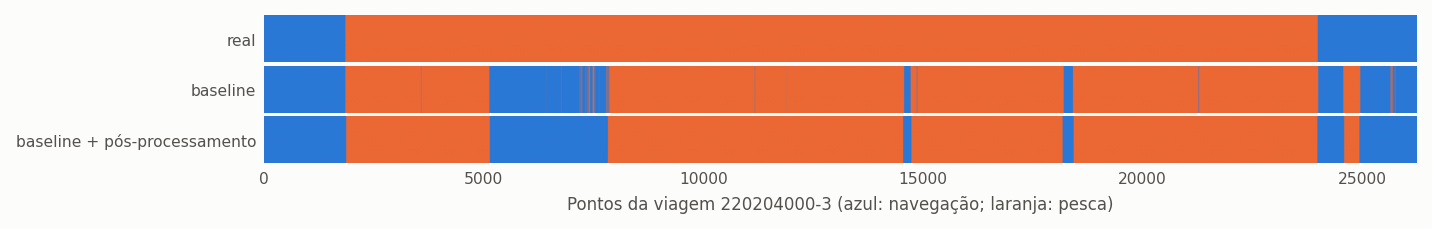
\includegraphics[width=0.9\linewidth]{validacao/220204000-3.png}\par}

26 239 pontos; segmentos de pesca reais: 1.

{\centering\small
\begin{tabular}{lrr}
\toprule
Linha & Exatidão & Segmentos de pesca previstos \\
\midrule
baseline & 87,0\,\% & 42 \\
baseline + pós-processamento & 86,6\,\% & 5 \\
\bottomrule
\end{tabular}\par}

\end{minipage}
\par

\par\smallskip\noindent\begin{minipage}{\linewidth}\setlength{\parskip}{3pt}
\hypertarget{219012671-2}{}\textbf{\large 219012671-2}\par

{\centering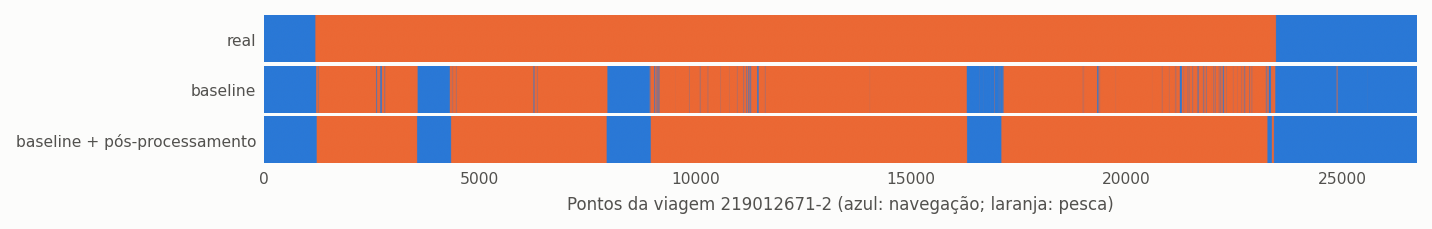
\includegraphics[width=0.9\linewidth]{validacao/219012671-2.png}\par}

26 727 pontos; segmentos de pesca reais: 1.

{\centering\small
\begin{tabular}{lrr}
\toprule
Linha & Exatidão & Segmentos de pesca previstos \\
\midrule
baseline & 87,7\,\% & 122 \\
baseline + pós-processamento & 89,6\,\% & 5 \\
\bottomrule
\end{tabular}\par}

\end{minipage}
\par

\par\smallskip\noindent\begin{minipage}{\linewidth}\setlength{\parskip}{3pt}
\hypertarget{220335000-2}{}\textbf{\large 220335000-2}\par

{\centering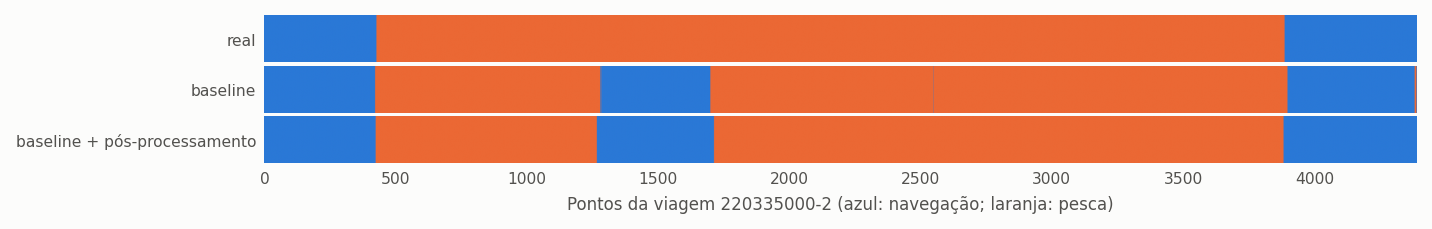
\includegraphics[width=0.9\linewidth]{validacao/220335000-2.png}\par}

4 389 pontos; segmentos de pesca reais: 1.

{\centering\small
\begin{tabular}{lrr}
\toprule
Linha & Exatidão & Segmentos de pesca previstos \\
\midrule
baseline & 89,9\,\% & 5 \\
baseline + pós-processamento & 89,7\,\% & 2 \\
\bottomrule
\end{tabular}\par}

\end{minipage}
\par

\par\smallskip\noindent\begin{minipage}{\linewidth}\setlength{\parskip}{3pt}
\hypertarget{219004343-1}{}\textbf{\large 219004343-1}\par

{\centering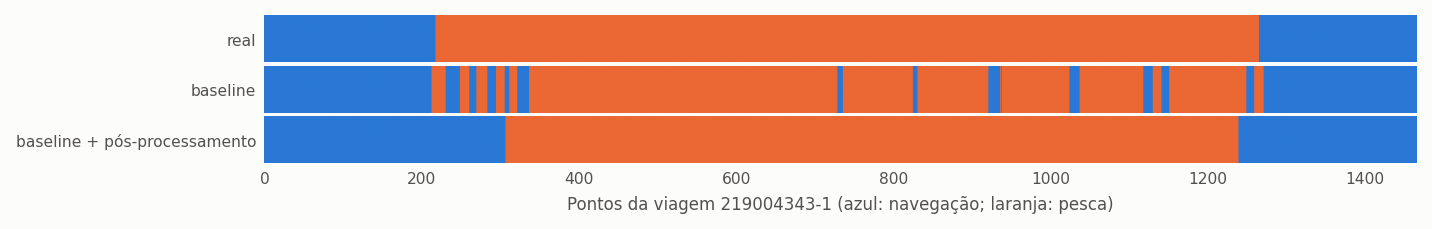
\includegraphics[width=0.9\linewidth]{validacao/219004343-1.png}\par}

1 466 pontos; segmentos de pesca reais: 1.

{\centering\small
\begin{tabular}{lrr}
\toprule
Linha & Exatidão & Segmentos de pesca previstos \\
\midrule
baseline & 90,2\,\% & 14 \\
baseline + pós-processamento & 92,2\,\% & 1 \\
\bottomrule
\end{tabular}\par}

\end{minipage}
\par

\par\smallskip\noindent\begin{minipage}{\linewidth}\setlength{\parskip}{3pt}
\hypertarget{219796000-2}{}\textbf{\large 219796000-2}\par

{\centering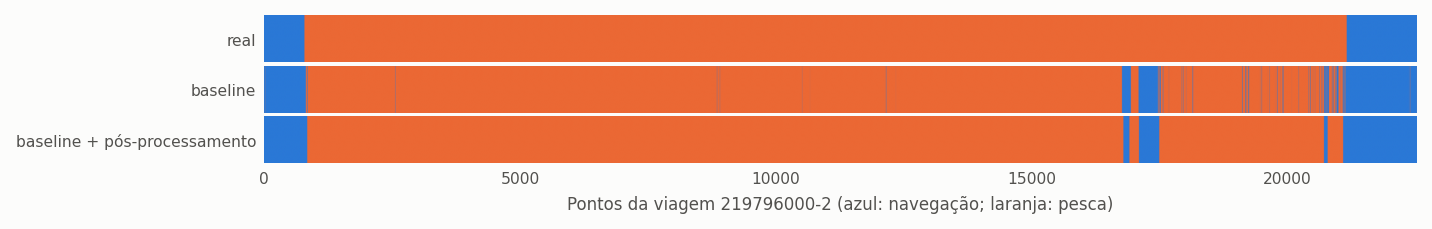
\includegraphics[width=0.9\linewidth]{validacao/219796000-2.png}\par}

22 522 pontos; segmentos de pesca reais: 1.

{\centering\small
\begin{tabular}{lrr}
\toprule
Linha & Exatidão & Segmentos de pesca previstos \\
\midrule
baseline & 95,4\,\% & 86 \\
baseline + pós-processamento & 96,8\,\% & 4 \\
\bottomrule
\end{tabular}\par}

\end{minipage}
\par

\par\smallskip\noindent\begin{minipage}{\linewidth}\setlength{\parskip}{3pt}
\hypertarget{219007027-2}{}\textbf{\large 219007027-2}\par

{\centering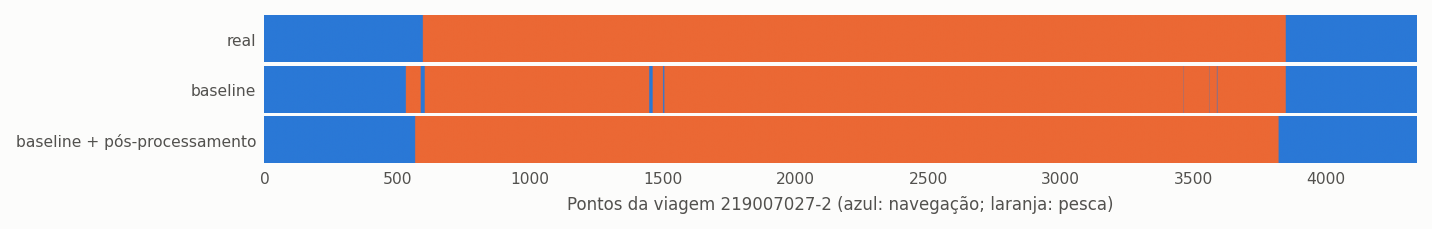
\includegraphics[width=0.9\linewidth]{validacao/219007027-2.png}\par}

4 340 pontos; segmentos de pesca reais: 1.

{\centering\small
\begin{tabular}{lrr}
\toprule
Linha & Exatidão & Segmentos de pesca previstos \\
\midrule
baseline & 98,0\,\% & 7 \\
baseline + pós-processamento & 98,7\,\% & 1 \\
\bottomrule
\end{tabular}\par}

\end{minipage}
\par

\par\smallskip\noindent\begin{minipage}{\linewidth}\setlength{\parskip}{3pt}
\hypertarget{219004128-2}{}\textbf{\large 219004128-2}\par

{\centering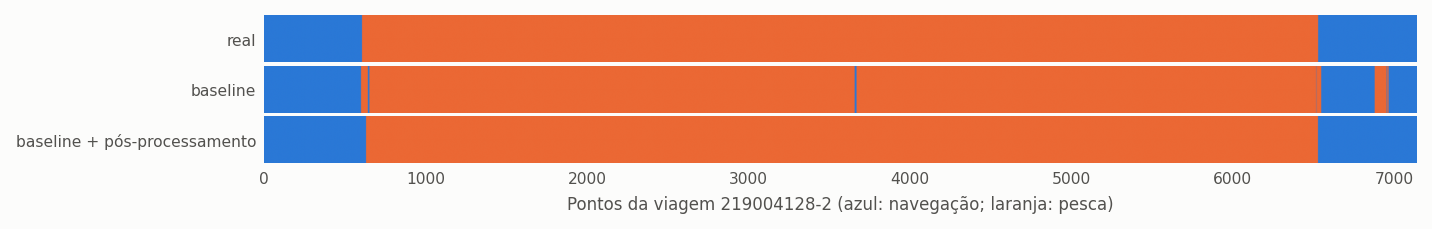
\includegraphics[width=0.9\linewidth]{validacao/219004128-2.png}\par}

7 139 pontos; segmentos de pesca reais: 1.

{\centering\small
\begin{tabular}{lrr}
\toprule
Linha & Exatidão & Segmentos de pesca previstos \\
\midrule
baseline & 98,2\,\% & 7 \\
baseline + pós-processamento & 99,6\,\% & 1 \\
\bottomrule
\end{tabular}\par}

\end{minipage}
\par

\par\smallskip\noindent\begin{minipage}{\linewidth}\setlength{\parskip}{3pt}
\hypertarget{220307000-3}{}\textbf{\large 220307000-3}\par

{\centering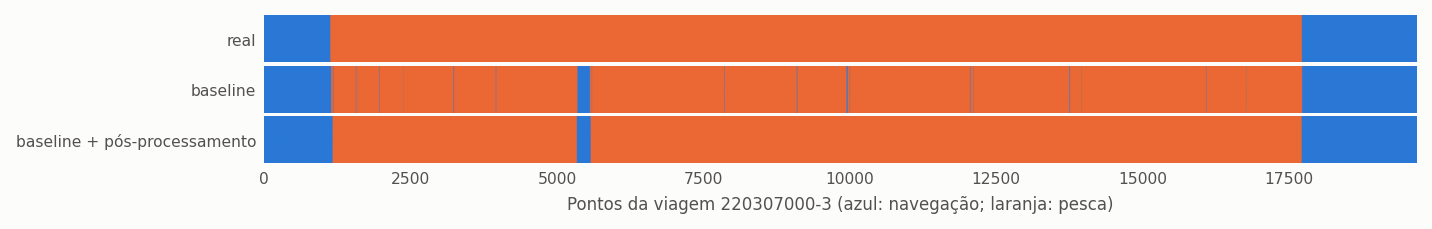
\includegraphics[width=0.9\linewidth]{validacao/220307000-3.png}\par}

19 677 pontos; segmentos de pesca reais: 1.

{\centering\small
\begin{tabular}{lrr}
\toprule
Linha & Exatidão & Segmentos de pesca previstos \\
\midrule
baseline & 98,2\,\% & 26 \\
baseline + pós-processamento & 98,6\,\% & 2 \\
\bottomrule
\end{tabular}\par}

\end{minipage}
\par

\par\smallskip\noindent\begin{minipage}{\linewidth}\setlength{\parskip}{3pt}
\hypertarget{219027026-2}{}\textbf{\large 219027026-2}\par

{\centering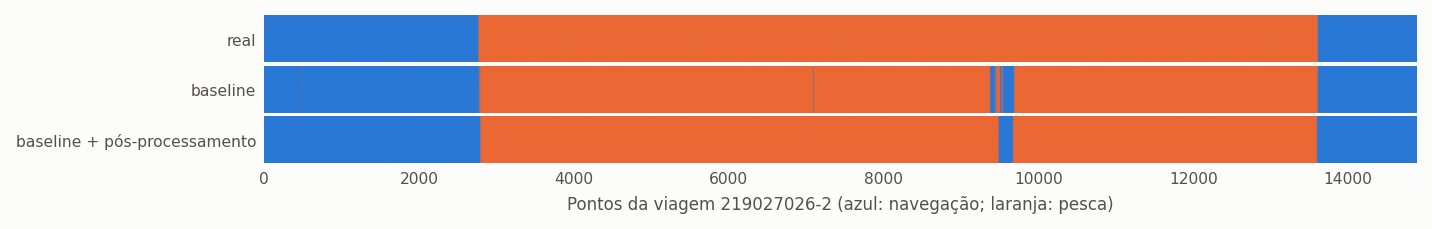
\includegraphics[width=0.9\linewidth]{validacao/219027026-2.png}\par}

14 880 pontos; segmentos de pesca reais: 1.

{\centering\small
\begin{tabular}{lrr}
\toprule
Linha & Exatidão & Segmentos de pesca previstos \\
\midrule
baseline & 98,2\,\% & 15 \\
baseline + pós-processamento & 98,5\,\% & 2 \\
\bottomrule
\end{tabular}\par}

\end{minipage}
\par

\par\smallskip\noindent\begin{minipage}{\linewidth}\setlength{\parskip}{3pt}
\hypertarget{211477000-2}{}\textbf{\large 211477000-2}\par

{\centering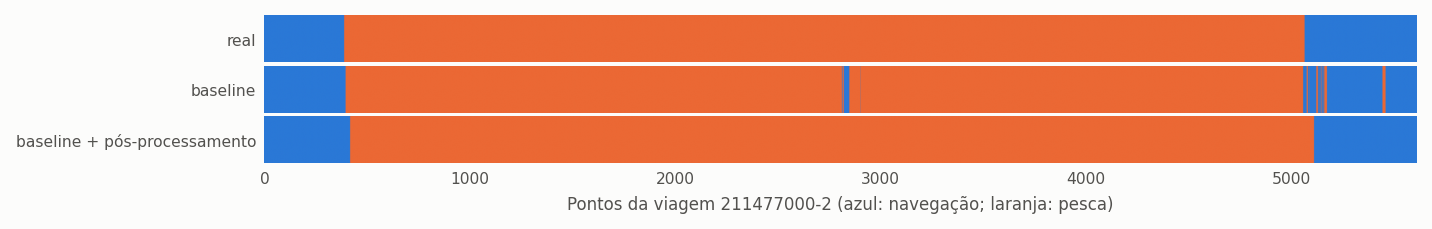
\includegraphics[width=0.9\linewidth]{validacao/211477000-2.png}\par}

5 610 pontos; segmentos de pesca reais: 1.

{\centering\small
\begin{tabular}{lrr}
\toprule
Linha & Exatidão & Segmentos de pesca previstos \\
\midrule
baseline & 98,3\,\% & 12 \\
baseline + pós-processamento & 98,7\,\% & 1 \\
\bottomrule
\end{tabular}\par}

\end{minipage}
\par

\par\smallskip\noindent\begin{minipage}{\linewidth}\setlength{\parskip}{3pt}
\hypertarget{219009738-2}{}\textbf{\large 219009738-2}\par

{\centering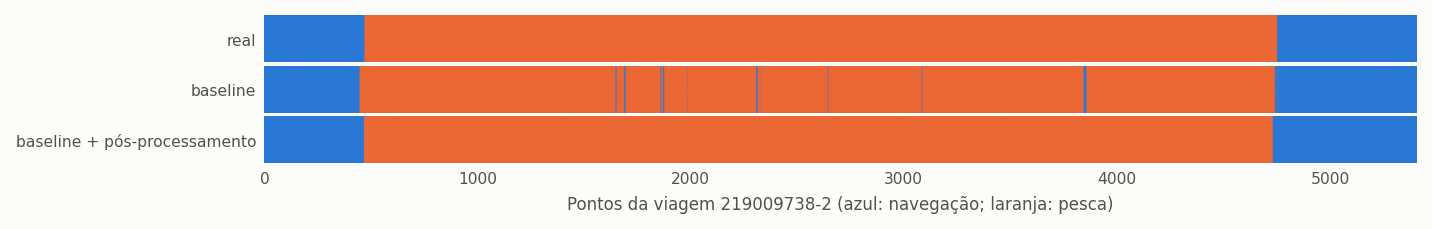
\includegraphics[width=0.9\linewidth]{validacao/219009738-2.png}\par}

5 406 pontos; segmentos de pesca reais: 1.

{\centering\small
\begin{tabular}{lrr}
\toprule
Linha & Exatidão & Segmentos de pesca previstos \\
\midrule
baseline & 98,4\,\% & 16 \\
baseline + pós-processamento & 99,6\,\% & 1 \\
\bottomrule
\end{tabular}\par}

\end{minipage}
\par

\par\smallskip\noindent\begin{minipage}{\linewidth}\setlength{\parskip}{3pt}
\hypertarget{219709000-2}{}\textbf{\large 219709000-2}\par

{\centering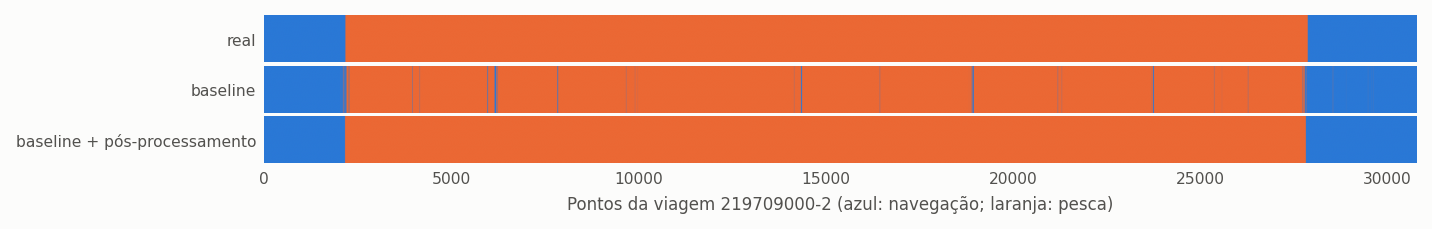
\includegraphics[width=0.9\linewidth]{validacao/219709000-2.png}\par}

30 772 pontos; segmentos de pesca reais: 1.

{\centering\small
\begin{tabular}{lrr}
\toprule
Linha & Exatidão & Segmentos de pesca previstos \\
\midrule
baseline & 98,6\,\% & 48 \\
baseline + pós-processamento & 99,8\,\% & 1 \\
\bottomrule
\end{tabular}\par}

\end{minipage}
\par

\par\smallskip\noindent\begin{minipage}{\linewidth}\setlength{\parskip}{3pt}
\hypertarget{220307000-4}{}\textbf{\large 220307000-4}\par

{\centering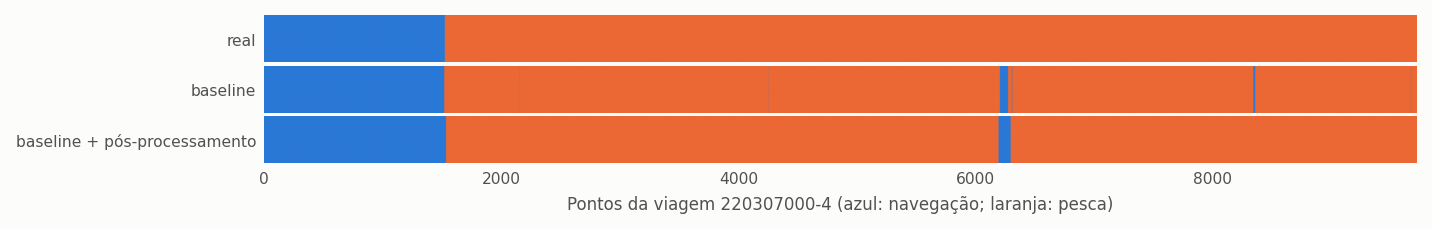
\includegraphics[width=0.9\linewidth]{validacao/220307000-4.png}\par}

9 722 pontos; segmentos de pesca reais: 1.

{\centering\small
\begin{tabular}{lrr}
\toprule
Linha & Exatidão & Segmentos de pesca previstos \\
\midrule
baseline & 99,0\,\% & 8 \\
baseline + pós-processamento & 98,8\,\% & 2 \\
\bottomrule
\end{tabular}\par}

\end{minipage}
\par

\par\smallskip\noindent\begin{minipage}{\linewidth}\setlength{\parskip}{3pt}
\hypertarget{219025740-2}{}\textbf{\large 219025740-2}\par

{\centering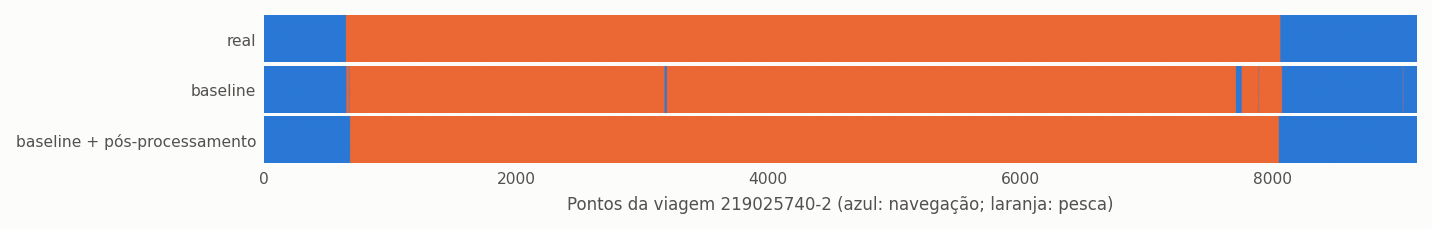
\includegraphics[width=0.9\linewidth]{validacao/219025740-2.png}\par}

9 146 pontos; segmentos de pesca reais: 1.

{\centering\small
\begin{tabular}{lrr}
\toprule
Linha & Exatidão & Segmentos de pesca previstos \\
\midrule
baseline & 99,0\,\% & 9 \\
baseline + pós-processamento & 99,5\,\% & 1 \\
\bottomrule
\end{tabular}\par}

\end{minipage}
\par

\par\smallskip\noindent\begin{minipage}{\linewidth}\setlength{\parskip}{3pt}
\hypertarget{220356000-3}{}\textbf{\large 220356000-3}\par

{\centering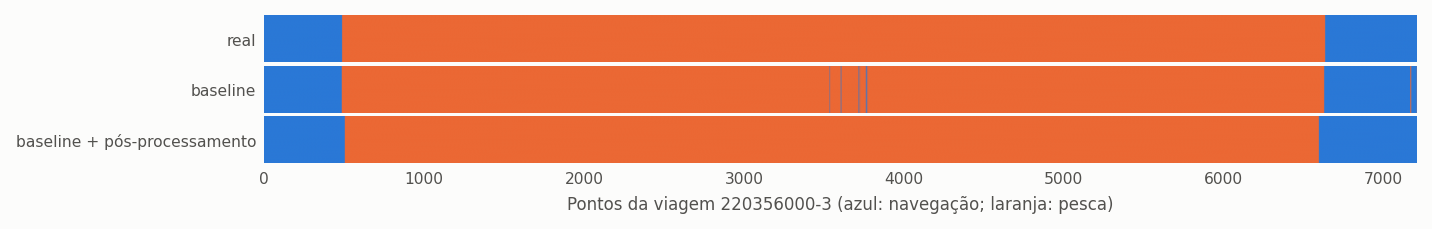
\includegraphics[width=0.9\linewidth]{validacao/220356000-3.png}\par}

7 205 pontos; segmentos de pesca reais: 1.

{\centering\small
\begin{tabular}{lrr}
\toprule
Linha & Exatidão & Segmentos de pesca previstos \\
\midrule
baseline & 99,5\,\% & 11 \\
baseline + pós-processamento & 99,2\,\% & 1 \\
\bottomrule
\end{tabular}\par}

\end{minipage}
\par

\par\smallskip\noindent\begin{minipage}{\linewidth}\setlength{\parskip}{3pt}
\hypertarget{219004128-4}{}\textbf{\large 219004128-4}\par

{\centering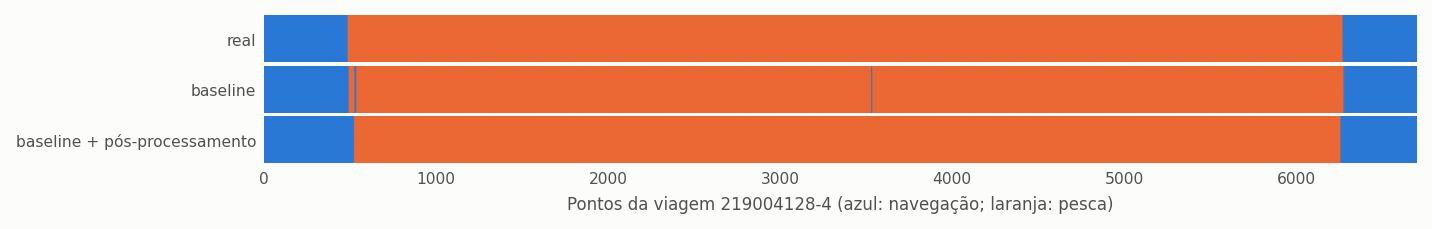
\includegraphics[width=0.9\linewidth]{validacao/219004128-4.png}\par}

6 700 pontos; segmentos de pesca reais: 1.

{\centering\small
\begin{tabular}{lrr}
\toprule
Linha & Exatidão & Segmentos de pesca previstos \\
\midrule
baseline & 99,6\,\% & 4 \\
baseline + pós-processamento & 99,3\,\% & 1 \\
\bottomrule
\end{tabular}\par}

\end{minipage}
\par

\par\smallskip\noindent\begin{minipage}{\linewidth}\setlength{\parskip}{3pt}
\hypertarget{220351000-2}{}\textbf{\large 220351000-2}\par

{\centering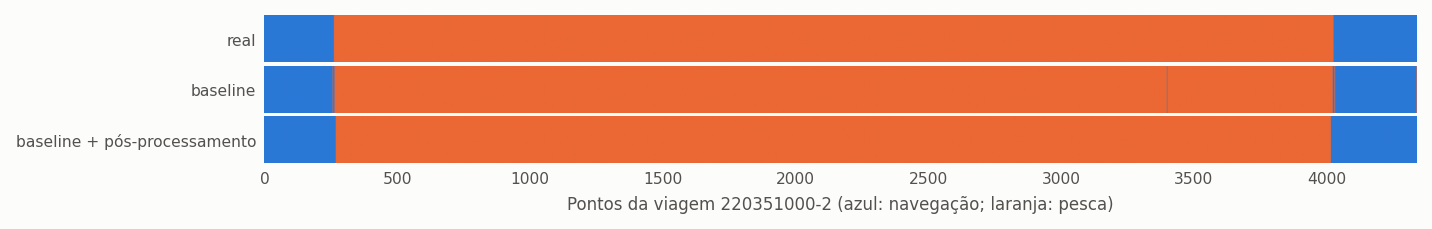
\includegraphics[width=0.9\linewidth]{validacao/220351000-2.png}\par}

4 338 pontos; segmentos de pesca reais: 1.

{\centering\small
\begin{tabular}{lrr}
\toprule
Linha & Exatidão & Segmentos de pesca previstos \\
\midrule
baseline & 99,7\,\% & 5 \\
baseline + pós-processamento & 99,6\,\% & 1 \\
\bottomrule
\end{tabular}\par}

\end{minipage}
\par

\end{document}
